% !TeX program = xelatex
% Overleaf: main document main.tex, compiler XeLaTeX.
\documentclass[UTF8,fontset=fandol,zihao=-4,a4paper,oneside]{ctexart}
\usepackage[left=2.54cm,right=2.54cm,top=2.40cm,bottom=2.40cm,headheight=15pt,headsep=0.6cm]{geometry}
\usepackage{graphicx,array,tabularx,longtable,multirow,booktabs}
\usepackage{tikz}
\usetikzlibrary{positioning,arrows.meta,calc,shapes.geometric}
\usepackage{enumitem,float,caption,fancyhdr,needspace,fvextra,xurl}
\usepackage[unicode,hidelinks,hypertexnames=false]{hyperref}
\hypersetup{pdftitle={第19组 校车管理系统中期报告},pdfauthor={许盛凯、赵凯彭},pdfsubject={现代软件工程课程设计}}
\setCJKfamilyfont{zhkai}[AutoFakeBold=2]{FandolKai-Regular.otf}
\setlength{\parindent}{2em}
\setlength{\parskip}{0pt}
\linespread{1.35}
\setlength{\emergencystretch}{2em}
\setlist{nosep,leftmargin=2em,topsep=3pt}
\ctexset{
 section={format=\songti\bfseries\zihao{-3},beforeskip=12pt,afterskip=8pt},
 subsection={format=\heiti\bfseries\zihao{4},beforeskip=10pt,afterskip=6pt},
 subsubsection={format=\kaishu\bfseries\zihao{-4},beforeskip=8pt,afterskip=5pt},
 contentsname={目\quad 录}}
\setcounter{tocdepth}{3}
\setcounter{secnumdepth}{3}
\pagestyle{fancy}
\fancyhf{}
\fancyhead[L]{\songti\zihao{5}《现代软件工程课程设计》中期报告}
\fancyfoot[C]{\small\thepage}
\renewcommand{\headrulewidth}{0.4pt}
\renewcommand{\footrulewidth}{0pt}
\DeclareCaptionFont{cns}{\zihao{5}\heiti}
\captionsetup{font=cns,labelfont=normalfont,labelsep=quad,skip=6pt}
\counterwithin{table}{section}
\counterwithin{figure}{section}
\renewcommand{\thetable}{\thesection.\arabic{table}}
\renewcommand{\thefigure}{\thesection.\arabic{figure}}
\newcolumntype{Y}{>{\raggedright\arraybackslash}X}
\newcolumntype{P}[1]{>{\raggedright\arraybackslash}p{#1}}
\setlength{\tabcolsep}{5pt}
\renewcommand{\arraystretch}{1.28}
\newcommand{\code}[1]{{\small\texttt{\nolinkurl{#1}}}}
\newcommand{\owner}[1]{\noindent\textbf{责任人：}#1\par}
\newcommand{\ReportDate}{2026 年 11 月 4 日}
% Group member student ID.
\newcommand{\ZhaoStudentId}{2023141230156}
\DefineVerbatimEnvironment{source}{Verbatim}{fontsize=\footnotesize,breaklines=true,breakanywhere=true,frame=single,framesep=5pt,baselinestretch=1.05}
\tikzset{box/.style={draw,rectangle,align=left,inner sep=5pt,font=\small},
 state/.style={draw,rounded corners=5pt,align=center,inner sep=7pt,font=\small},
 flow/.style={-{Stealth[length=2mm]},semithick},
 lifeline/.style={dashed,gray},
 smalllabel/.style={font=\footnotesize,fill=white,inner sep=2pt}}
\begin{document}
\begin{titlepage}
\thispagestyle{empty}
\centering
\vspace*{1.8cm}
{\songti\bfseries\fontsize{24}{34}\selectfont《现代软件工程课程设计》\par 中期报告\par}
\vspace{1.0cm}
{\heiti\zihao{2}校车管理系统\par}
\vspace{2.3cm}
{\zihao{4}
\begin{tabular}{|>{\centering\arraybackslash}p{3.0cm}|>{\centering\arraybackslash}p{5.4cm}|>{\centering\arraybackslash}p{3.3cm}|}
\hline
小组编号 & \multicolumn{2}{c|}{第19组}\\[10pt]\hline
\multirow{3}{*}{小组成员} & 学号 & 姓名\\[10pt]\cline{2-3}
 & 2024141460445 & 许盛凯\\[10pt]\cline{2-3}
 & \ZhaoStudentId & 赵凯彭\\[10pt]\hline
\end{tabular}}
\vfill
{\songti\zihao{4}提交报告时间：\ReportDate\par}
\vspace*{1.6cm}
\end{titlepage}
\pagestyle{empty}
\tableofcontents
\clearpage
\pagestyle{fancy}
\pagenumbering{arabic}
\section{已实现功能}
本项目面向校园通勤中的乘车预约、司机执行任务和车辆调度需求，采用 Flutter 单工程构建普通用户端、司机端与后台管理端。现阶段已完成角色入口、核心数据模型和三端业务原型，能够在内置演示数据上运行主要操作流程。小组目前已实现的功能及责任人如表\ref{tab:functions}所示。

\begin{table}[H]
\centering\small
\caption{已实现功能列表}\label{tab:functions}
\begin{tabularx}{\linewidth}{|P{2.0cm}|Y|P{1.6cm}|}
\hline
\centering 类别 & \centering 功能 & \centering\arraybackslash 责任人\\\hline
公共入口 & 演示账号登录、入口切换、角色匹配与路由重定向 & 许盛凯\\\hline
普通用户端 & 浏览车次、查看余座、选择座位并创建预约 & 许盛凯\\\hline
普通用户端 & 查看与筛选个人预约、取消预约和信用扣分 & 许盛凯\\\hline
普通用户端 & 模拟支付、信用等级展示、本地通知中心 & 许盛凯\\\hline
司机端 & 查看派车任务、乘客名单和上车点 & 赵凯彭\\\hline
司机端 & 开始任务、到站完成、单个活动任务约束 & 赵凯彭\\\hline
司机端 & 每5秒生成模拟位置记录、展示位置共享状态 & 赵凯彭\\\hline
司机端 & 日、周、月维度切换及预置任务统计展示 & 赵凯彭\\\hline
后台管理端 & 车辆与司机信息维护、绑定校验和删除限制 & 许盛凯\\\hline
后台管理端 & 人工调度、规则辅助建议、人工确认生效 & 许盛凯\\\hline
后台管理端 & 模拟车辆位置、示例 ETA 与历史分析面板 & 许盛凯\\\hline
工程验证 & 预约、任务、调度等关键规则的测试与整理 & 许盛凯、赵凯彭\\\hline
\end{tabularx}
\end{table}

目前界面层通过 Riverpod 读取和更新业务状态，GoRouter 管理三类工作台的访问入口，Mock Repository 提供初始车次、任务、车辆和需求数据。模型、状态控制和页面展示已分离，后续可以在保留主要界面交互的基础上替换数据来源。

当前阶段成果以可运行原型为范围。支付操作更新本地支付状态，位置共享使用定时生成的坐标，后台辅助调度采用规则匹配；各端演示数据尚未通过统一服务端同步。数据持久化、真实支付、GPS 采集和实时通信是下一阶段需要继续设计与联调的内容。

\clearpage
\section{建模与构建}
本章从表\ref{tab:functions}中选择三个代表功能展开：许盛凯负责的乘客预约选座、后台辅助调度，以及赵凯彭负责的司机任务与位置共享。每个功能均按场景建模、类建模、功能建模/行为建模、代码结构及说明、界面截图的顺序给出阶段结果。建模围绕现有 Dart 类和控制器方法展开，突出业务规则与实现之间的对应关系。

\subsection{功能一 乘客预约选座与订单管理}
\owner{许盛凯}
该功能将车次容量、座位占用、重复预约和订单状态约束集中到状态控制器，是乘客端最主要的交互流程。其难点在于页面显示的可选座位必须与创建预约时的校验保持一致，取消操作还会同时影响座位、信用分和通知。

\subsubsection{场景建模}
\begin{table}[H]\centering\small
\caption{乘客预约选座用例描述}
\begin{tabularx}{\linewidth}{|P{2cm}|Y|}\hline
用例名称 & UC-P01 预约车次并选择座位\\\hline
参与者 & 已登录的普通用户\\\hline
前置条件 & 用户进入普通用户工作台；目标车次处于待发车状态且发车时间晚于当前时间。\\\hline
触发事件 & 用户在车次卡片点击预约，进入选座对话框。\\\hline
基本流程 & （1）查看路线、时间、费用和余座；（2）打开选座界面；（3）选择可用座位；（4）确认预约；（5）控制器校验车次、余座、重复预约和座位有效性；（6）创建待发车、待支付的预约；（7）刷新列表并生成预约通知。\\\hline
异常流程 & 车次不可预约、余座为零、同一用户已有该车次有效预约或所选座位不可用时，返回具体原因，不新增预约。\\\hline
后置条件 & 新预约进入个人预约列表；该座位从可用座位集合中移除，车次显示余座相应减少。\\\hline
关联操作 & 模拟支付更新支付状态；发车前取消预约释放占座并扣减信用分。\\\hline
\end{tabularx}\end{table}
预约、支付和取消分别由独立操作触发。订单的业务状态与支付状态分开保存：支付成功后订单仍为待发车状态，不将“已支付”作为行程结束。取消仅允许待发车预约，且车次不能已发车。

\subsubsection{类建模}
图\ref{fig:passenger-class}保留与预约直接相关的核心字段。用户与车次通过预约关联，支付记录通过预约标识与订单关联；控制器管理状态，页面只调用操作并展示结果。
\begin{figure}[H]\centering
\begin{tikzpicture}[x=1cm,y=1cm]
\node[box,text width=5.9cm] (trip) at (0,0) {\textbf{TripModel}\par\rule{5.7cm}{0.3pt}\par\code{id, departureTime, totalSeats}\par\code{bookedSeats, fare, status}\par\code{isBookable}};
\node[box,text width=5.9cm] (user) at (7.3,0) {\textbf{UserModel}\par\rule{5.7cm}{0.3pt}\par\code{id, name, phone}\par\code{role, creditScore}\par 用户身份与信用状态};
\node[box,text width=5.9cm] (booking) at (0,-4.0) {\textbf{BookingModel}\par\rule{5.7cm}{0.3pt}\par\code{id, userId, tripId, seatNo}\par\code{status, fare, paymentStatus}\par\code{isActive, canPay, copyWith()}};
\node[box,text width=5.9cm] (pay) at (7.3,-4.0) {\textbf{PaymentModel}\par\rule{5.7cm}{0.3pt}\par\code{id, bookingId, amount}\par\code{method, status}\par\code{createdAt, completedAt}};
\draw (trip.south)--node[font=\scriptsize,right,pos=.15]{1}node[font=\scriptsize,right,pos=.85]{0..*}(booking.north);
\draw (user.south)--node[font=\scriptsize,right,pos=.15]{1}node[font=\scriptsize,right,pos=.85]{0..*}(booking.north east);
\draw (booking.east)--node[font=\scriptsize,above]{1\quad 0..*}(pay.west);
\end{tikzpicture}
\caption{乘客预约核心类模型（字段节选，关联通过标识保存）}\label{fig:passenger-class}
\end{figure}

\noindent\textbf{模型约束。}有效预约由\code{BookingModel.isActive}判定，其条件是业务状态为\code{pending}。\code{TripModel.isBookable}同时检查车次状态与发车时间。Mock 数据中\code{bookedSeats}表示初始化时已有的占用座位，新增预约单独记录，因此计算余座时需要扣除两部分。

\subsubsection{功能建模/行为建模}
图\ref{fig:passenger-sequence}展示从用户确认选座到状态刷新和本地通知的关键顺序。初始数据由仓库提供，实际创建预约时直接读取当前内存状态，无网络请求。
\begin{figure}[H]\centering
\begin{tikzpicture}[x=1cm,y=1cm,font=\small]
\node[box,align=center,text width=1.35cm] (u) at (0,0) {乘客};
\node[box,align=center,text width=2cm] (ui) at (3.0,0) {预约页面};
\node[box,align=center,text width=2.8cm] (c) at (7.0,0) {预约控制器};
\node[box,align=center,text width=2.0cm] (n) at (11.5,0) {本地通知状态};
\foreach \a in {u,ui,c,n} \draw[lifeline] (\a.south)--+(0,-6.8);
\draw[flow] (0,-1)--node[above,smalllabel]{选座并确认}(3,-1);
\draw[flow] (3,-2)--node[above,smalllabel]{createBooking(...)}(7,-2);
\draw[flow] (7,-2.55)--(7.8,-2.55)--node[right,font=\footnotesize,align=left]{校验车次、容量、\\重复预约、座位}(7.8,-3.5)--(7,-3.5);
\node[box,text width=5.6cm,font=\footnotesize,align=center] at (3.0,-4.0) {校验失败：返回原因，页面提示，不新增预约};
\draw[flow] (7,-4.8)--(8,-4.8)--node[right,font=\footnotesize]{创建预约并替换状态}(8,-5.4)--(7,-5.4);
\draw[flow] (7,-5.85)--node[above,smalllabel]{push 预约通知}(11.5,-5.85);
\draw[flow,dashed] (7,-6.6)--node[above,smalllabel]{返回操作结果 / 状态变化刷新 UI}(3,-6.6);
\end{tikzpicture}
\caption{预约创建的关键交互顺序}\label{fig:passenger-sequence}
\end{figure}

余座和座位集合的计算规则为：
\[
 R=T-B-\left|\{b\mid b.tripId=t.id\land b.isActive\}\right|,
\]
其中 $T$ 为车次总座位数，$B$ 为初始化占用数。可选座位从 $B+1$ 到 $T$ 枚举，再移除有效预约已使用的座位号。取消后预约不再属于有效集合，因此该座位可重新选择。

取消时，距发车时间不超过120分钟扣5分，其余扣2分；已发车时直接拒绝取消。模拟支付单独经历待支付、支付中和已支付状态。以上规则在控制器中统一处理，避免不同页面各自维护一套判断。

\subsubsection{代码结构及说明}
\begin{table}[H]\centering\small
\caption{预约功能代码结构与职责}
\begin{tabularx}{\linewidth}{|P{2.1cm}|Y|}\hline
层次 & 文件与职责\\\hline
页面层 & \code{lib/features/passenger/presentation/passenger_home_page.dart}：车次卡片、选座对话框、预约列表、取消确认与支付界面。\\\hline
状态层 & \code{lib/features/passenger/booking/providers/passenger_booking_provider.dart}：管理车次、预约、支付及业务操作结果。\\\hline
数据层 & \code{lib/features/passenger/booking/data/mock_passenger_repository.dart}：提供初始车次和预约。\\\hline
模型与公共状态 & \code{lib/core/models/booking_model.dart}、\code{trip_model.dart}、\code{payment_model.dart}；信用与通知分别由认证状态和通知状态管理。\\\hline
\end{tabularx}\end{table}

\noindent\textbf{核心方法。}\code{createBooking}依次检查业务条件，构造\code{BookingModel}，再以新列表更新状态；\code{cancelBooking}更新预约、扣减信用分并写入通知；\code{payBooking}创建支付记录并通过模拟延时更新结果。下面摘录创建预约的主要校验，省略返回消息和对象构造：
\begin{source}
if (!trip.isBookable) return failure;
if (state.remainingSeatsForTrip(tripId) <= 0) return failure;
if (state.hasActiveBooking(userId: userId, tripId: tripId)) {
  return failure;
}
if (!state.availableSeatsForTrip(tripId).contains(seatNo)) {
  return failure;
}
// Create BookingModel; replace state; push local notification.
\end{source}
\noindent 上述为控制流程摘要，\code{failure}代表实际代码中带具体消息的\code{BookingActionResult}。实现通过不可变对象与列表替换触发页面刷新，页面不直接修改模型字段。

\noindent\textbf{阶段验证。}已有测试覆盖创建预约、取消和模拟支付，以及同车次重复预约、重复取消和不可取消状态等规则。测试文件为\code{test/widget_test.dart}与\code{test/business_rule_test.dart}。下一阶段需要增加并发占座、支付与取消交叉操作的验证，并在共享服务端接入后使用事务保证跨设备座位一致性。

\clearpage
\subsubsection{界面截图}
\begin{figure}[H]\centering
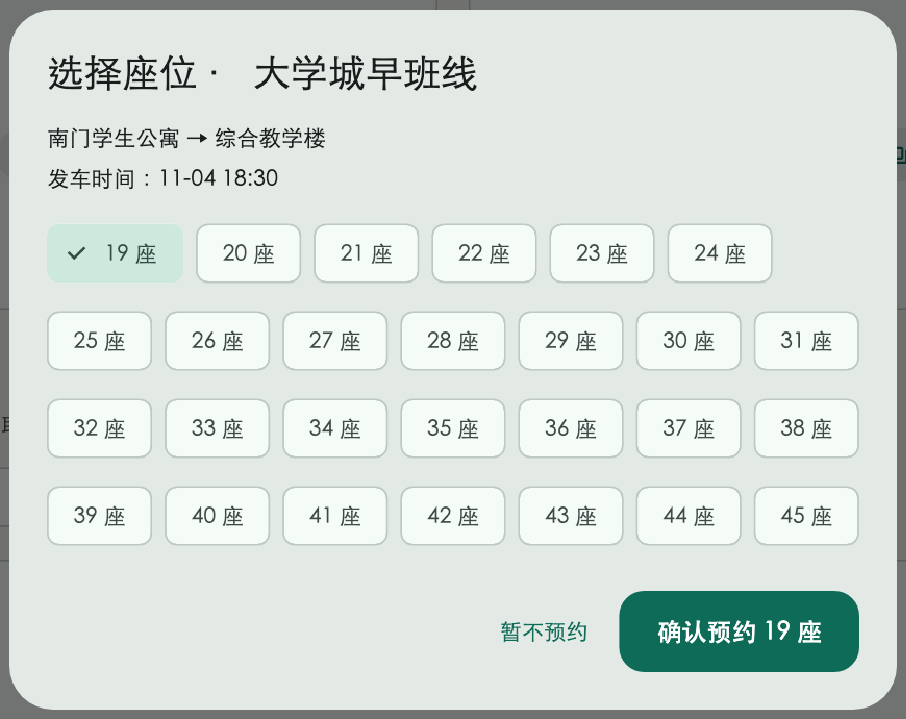
\includegraphics[width=12cm,height=0.64\textheight,keepaspectratio]{figures/passenger.pdf}
\caption{乘客选择19号座位并确认预约的运行界面}\label{fig:passenger-screen}
\end{figure}

界面将路线、发车时间、票价和余座放在同一车次卡片中，选座对话框提供明确的座位编号与可选状态。确认后，用户可以在“我的预约”中继续完成支付或取消，相关状态由同一预约模型驱动。

本阶段已完成从车次浏览到预约创建的本地交互流程，并补充了取消、信用和支付状态展示。后续将优先完善错误反馈和边界测试，再对接持久化与统一认证，保持预约规则在三端共享数据后的稳定性。

\clearpage
\subsection{功能二 后台人工调度与规则辅助调度}
\owner{许盛凯}
后台调度需要把待出行需求与车辆、司机联系起来。该功能的代表性在于同一操作会改变需求分配、方案确认和车辆运行状态，并要求在生成建议后保留人工确认环节，避免仅生成方案就直接占用运力。

\subsubsection{场景建模}
\begin{table}[H]\centering\small
\caption{后台规则辅助调度用例描述}
\begin{tabularx}{\linewidth}{|P{2cm}|Y|}\hline
用例名称 & UC-A01 生成并确认辅助调度方案\\\hline
参与者 & 已登录后台工作台的管理员\\\hline
前置条件 & 存在待调度需求；车辆和司机信息已录入；规则辅助调度使用空闲且已绑定司机的车辆。\\\hline
触发事件 & 管理员点击界面中的“AI 辅助调度”操作。\\\hline
基本流程 & （1）读取待调度需求；（2）按乘客人数降序排列；（3）依次寻找容量足够的候选车辆及绑定司机；（4）生成待确认建议并展示装载率；（5）管理员核对方案；（6）确认时再次检查关键数据与车辆状态；（7）更新方案、需求、车辆和后台位置记录。\\\hline
异常流程 & 没有候选车辆、没有待调度需求或无法覆盖任何需求时返回提示；方案不存在、已确认或车辆已不空闲时拒绝确认。\\\hline
后置条件 & 成功确认的方案标记为已确认，对应需求为已调度，车辆为运行中，后台新增该车辆位置记录。\\\hline
替代流程 & 管理员手工选择需求、车辆和司机，校验空闲状态、绑定关系与座位容量后生成待确认方案。\\\hline
\end{tabularx}\end{table}
界面沿用“AI 辅助调度”的功能名称，当前实现为可解释的规则匹配。管理员可查看建议并人工确认，现阶段没有调用外部大模型，也没有全局最优调度求解过程。

\subsubsection{类建模}
图\ref{fig:dispatch-class}将需求与调度结果分成两个实体。方案保存需求、车辆和司机的标识以及当次装载率，避免将需求数据直接当作已执行任务。
\begin{figure}[H]\centering
\begin{tikzpicture}[x=1cm,y=1cm]
\node[box,text width=5.9cm] (demand) at (0,0) {\textbf{DispatchDemandModel}\par\rule{5.7cm}{0.3pt}\par\code{id, routeName, passengerCount}\par\code{departureTime, status}};
\node[box,text width=5.9cm] (plan) at (7.3,0) {\textbf{DispatchPlanModel}\par\rule{5.7cm}{0.3pt}\par\code{demandId, vehicleId, driverId}\par\code{loadRate, isConfirmed}\par\code{isAiGenerated}};
\node[box,text width=5.9cm] (v) at (0,-4.0) {\textbf{VehicleModel}\par\rule{5.7cm}{0.3pt}\par\code{id, plateNo, model}\par\code{seatCount, status}};
\node[box,text width=5.9cm] (dr) at (7.3,-4.0) {\textbf{AdminDriverModel}\par\rule{5.7cm}{0.3pt}\par\code{id, name, phone, licenseNo}\par\code{boundVehicleId?}};
\draw (demand.east)--node[font=\scriptsize,above]{1\quad 0..*}(plan.west);
\draw (plan.south west)--node[font=\scriptsize,above,sloped,pos=.25]{0..*}node[font=\scriptsize,above,sloped,pos=.85]{1}(v.north east);
\draw (plan.south)--node[font=\scriptsize,right,pos=.2]{0..*}node[font=\scriptsize,right,pos=.8]{1}(dr.north);
\draw[dashed] (v.east)--node[font=\scriptsize,above]{绑定}(dr.west);
\end{tikzpicture}
\caption{后台调度核心类模型（历史方案可多次引用资源）}\label{fig:dispatch-class}
\end{figure}

\noindent\textbf{类之间的关系。}\code{DispatchDemandModel}保存路线、人数、时间和需求状态；\code{DispatchPlanModel}保存匹配结果、生成方式与确认标记；\code{VehicleModel}描述车辆容量与运行状态；\code{AdminDriverModel.boundVehicleId}描述可选的车辆绑定。\code{AdminController}统一完成查找、校验和状态替换。

\subsubsection{功能建模/行为建模}
图\ref{fig:dispatch-flow}概括建议生成和确认的活动流程。生成阶段使用集合记录本批次已匹配的车辆，防止一辆车在同一批建议中被重复使用；未找到适配车辆的需求保留待调度状态。
\begin{figure}[H]\centering
\begin{tikzpicture}[node distance=0.45cm,font=\small]
\node[state,text width=8cm,inner sep=4pt] (a) {读取空闲且绑定司机的候选车辆};
\node[state,text width=8cm,inner sep=4pt,below=of a] (b) {待调度需求按人数降序排序};
\node[state,text width=8cm,inner sep=4pt,below=of b] (c) {依次匹配容量足够且本批尚未使用的车辆};
\node[state,text width=8cm,inner sep=4pt,below=of c] (d) {生成待确认建议，记录车辆使用情况\par 无法匹配的需求保持待调度};
\node[state,text width=8cm,inner sep=4pt,below=of d] (e) {展示路线、司机、车辆和装载率\par 等待管理员确认};
\node[state,text width=8cm,inner sep=4pt,below=of e] (f) {复核方案、关联数据与车辆空闲状态};
\node[state,text width=8cm,inner sep=4pt,below=of f] (g) {确认方案；需求已调度；车辆运行中\par 建立后台车辆位置记录};
\foreach \s/\t in {a/b,b/c,c/d,d/e,e/f,f/g} \draw[flow] (\s)--(\t);
\node[box,align=center,text width=2.15cm,right=1.0cm of b] (err) {无候选或\par 无待调度需求\par 返回提示};
\draw[flow] (a.east)-| (err.north);
\draw[flow] (b.east)--(err.west);
\node[box,align=center,text width=2.15cm,right=1.0cm of f] (err2) {复核失败\par 拒绝确认\par 提示原因};
\draw[flow] (f.east)--(err2.west);
\end{tikzpicture}
\caption{规则辅助调度与人工确认活动流程}\label{fig:dispatch-flow}
\end{figure}

规则按需求人数降序逐项匹配，选择候选集合中首个容量足够且本批未用的车辆。装载率按“需求人数/车辆座位数”计算。该规则便于解释和演示，但结果会受候选车辆顺序影响，尚未覆盖多车拆分、时间冲突和路线成本等约束。

确认操作与建议生成分开：确认时检查方案是否存在、是否已确认、需求/车辆/司机是否仍存在及车辆是否空闲。成功后一次性替换后台状态中的相关列表。后续接入共享服务端时，还需对需求重复分配、司机冲突和并发确认进行更完整的事务校验。

\subsubsection{代码结构及说明}
\begin{table}[H]\centering\small
\caption{调度功能代码结构与职责}
\begin{tabularx}{\linewidth}{|P{2.1cm}|Y|}\hline
层次 & 文件与职责\\\hline
页面层 & \code{lib/features/admin/presentation/admin_home_page.dart}：待调度需求、人工调度对话框、建议卡片和确认入口。\\\hline
状态层 & \code{lib/features/admin/providers/admin_provider.dart}：车辆司机维护、调度建议生成、方案确认和位置模拟。\\\hline
数据层 & \code{lib/features/admin/data/mock_admin_repository.dart}：提供演示车辆、司机、需求、位置与分析快照。\\\hline
模型层 & \code{lib/core/models/dispatch_model.dart}、\code{vehicle_model.dart}、\code{admin_driver_model.dart}和\code{vehicle_location_model.dart}。\\\hline
\end{tabularx}\end{table}

\noindent\textbf{关键操作。}\code{generateAiDispatchPlans}生成规则建议；\code{createManualDispatchPlan}处理人工选择；\code{confirmDispatchPlan}执行确认。规则匹配的核心片段如下：
\begin{source}
final sortedDemands = [...state.pendingDispatchDemands]
  ..sort((a, b) => b.passengerCount.compareTo(a.passengerCount));
final usedVehicleIds = <String>{};
for (final demand in sortedDemands) {
  final pair = candidates.where((item) {
    return !usedVehicleIds.contains(item.vehicle.id) &&
        item.vehicle.seatCount >= demand.passengerCount;
  }).firstOrNull;
  if (pair == null) continue;
  usedVehicleIds.add(pair.vehicle.id);
  // Build one pending plan with demand, vehicle and driver.
}
\end{source}
\noindent 片段中的候选集合由\code{_availableVehicleDriverPairs}构造。方法只纳入空闲且已有绑定司机的车辆；人工调度则允许在通过绑定检查的情况下选择未绑定司机，确认时再建立绑定。

\noindent\textbf{阶段验证。}已有测试覆盖人工方案、建议生成、确认，以及无可用车辆和座位不足等失败分支。当前确认只更新后台模块的内存数据，尚不会自动向乘客端创建车次或向司机端推送任务。下一阶段将统一这三种业务对象的标识与接口，并补充重复需求、车辆状态变化和司机占用冲突的测试。

\clearpage
\subsubsection{界面截图}
\begin{figure}[H]\centering
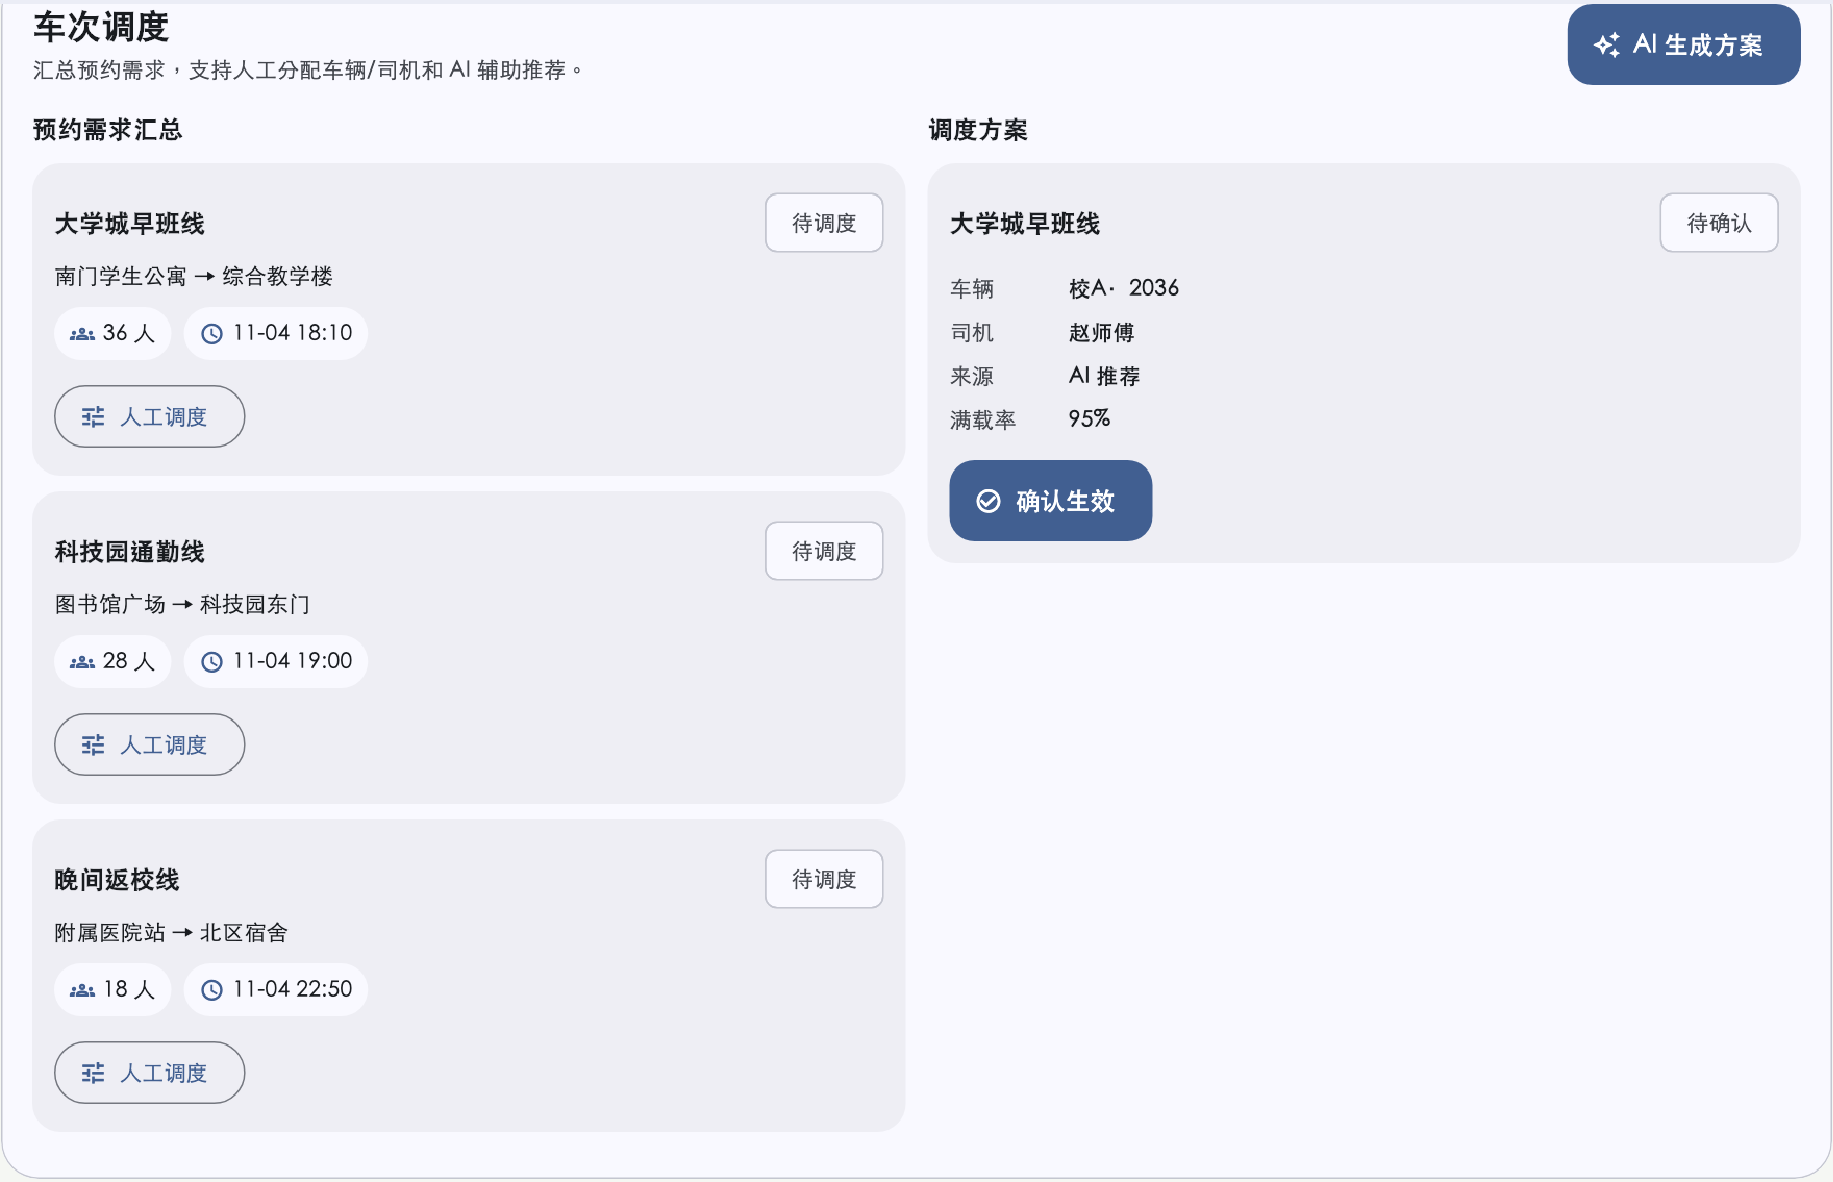
\includegraphics[width=\linewidth,height=0.64\textheight,keepaspectratio]{figures/dispatch.pdf}
\caption{后台生成调度建议并等待人工确认的运行界面}\label{fig:dispatch-screen}
\end{figure}

调度界面将需求信息与建议结果分区展示。管理员可以核对路线、发车时间、乘客人数、车辆、司机与装载率，再点击确认；人工调度则通过对话框逐项选择资源，使规则建议与人工处理共用同一确认流程。

现阶段后台已经形成“维护运力—生成方案—人工确认—查看状态”的本地操作流程。后续重点是完善确认前的约束复核，并将确认结果映射为统一车次和司机任务，逐步完成真实数据条件下的跨端联调。

\clearpage
\subsection{功能三 司机任务执行与模拟位置共享}
\owner{赵凯彭}
司机端围绕一次行程组织任务列表、乘客名单、上车点和位置共享状态。其主要难点是协调任务生命周期与定时器生命周期：发车后生成位置记录，到站后停止生成，并保证同一时刻只有一个活动任务。

\subsubsection{场景建模}
\begin{table}[H]\centering\small
\caption{司机执行任务与位置共享用例描述}
\begin{tabularx}{\linewidth}{|P{2cm}|Y|}\hline
用例名称 & UC-D01 执行派车任务并共享模拟位置\\\hline
参与者 & 已登录司机工作台的司机\\\hline
前置条件 & 已加载演示任务；目标任务尚未完成；当前没有活动任务。\\\hline
触发事件 & 司机核对任务后点击开始任务。\\\hline
基本流程 & （1）查看车次、路线、发车时间和乘客数；（2）展开乘客名单及上车点；（3）开始任务；（4）任务状态改为行程中并记录活动任务标识；（5）立即生成首条位置，此后每5秒生成一条；（6）到站后完成任务；（7）任务改为已完成，停止定时器并清除活动任务。\\\hline
异常流程 & 已有活动任务、任务不存在或任务已完成时拒绝开始；没有活动任务时不能完成任务。\\\hline
后置条件 & 任务状态与位置共享状态一致；已完成任务不能再次发车；已有位置记录保留供页面查看。\\\hline
关联操作 & 切换日、周、月统计维度，查看对应预置统计数据。\\\hline
\end{tabularx}\end{table}
界面中的位置上报通过本地坐标序列模拟。5秒代表定时生成记录的间隔，能够用于检查状态更新和交互流程；真实 GPS 权限、后台定位、网络上传和管理员订阅需要在后续联调中完成。

\subsubsection{类建模}
图\ref{fig:driver-class}以任务状态为中心组织乘客上车信息与位置记录。任务内包含乘客列表，位置记录通过车辆标识对应车辆；控制器保存活动任务标识和位置列表。
\begin{figure}[H]\centering
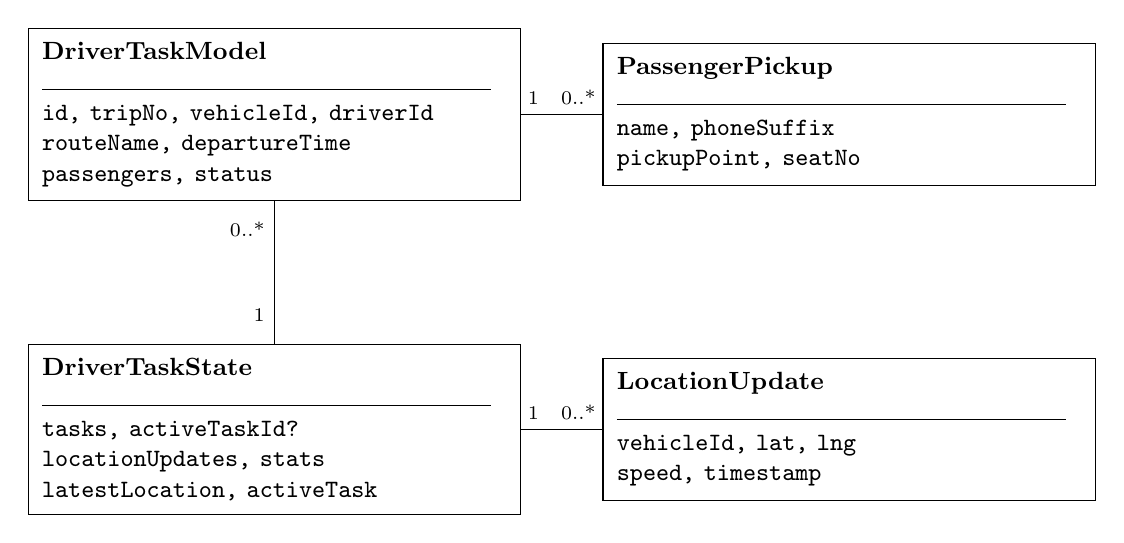
\begin{tikzpicture}[x=1cm,y=1cm]
\node[box,text width=5.9cm] (task) at (0,0) {\textbf{DriverTaskModel}\par\rule{5.7cm}{0.3pt}\par\code{id, tripNo, vehicleId, driverId}\par\code{routeName, departureTime}\par\code{passengers, status}};
\node[box,text width=5.9cm] (pickup) at (7.3,0) {\textbf{PassengerPickup}\par\rule{5.7cm}{0.3pt}\par\code{name, phoneSuffix}\par\code{pickupPoint, seatNo}};
\node[box,text width=5.9cm] (state) at (0,-4.0) {\textbf{DriverTaskState}\par\rule{5.7cm}{0.3pt}\par\code{tasks, activeTaskId?}\par\code{locationUpdates, stats}\par\code{latestLocation, activeTask}};
\node[box,text width=5.9cm] (loc) at (7.3,-4.0) {\textbf{LocationUpdate}\par\rule{5.7cm}{0.3pt}\par\code{vehicleId, lat, lng}\par\code{speed, timestamp}};
\draw (task.east)--node[font=\scriptsize,above]{1\quad 0..*}(pickup.west);
\draw (state.north)--node[font=\scriptsize,left,pos=.2]{1}node[font=\scriptsize,left,pos=.8]{0..*}(task.south);
\draw (state.east)--node[font=\scriptsize,above]{1\quad 0..*}(loc.west);
\end{tikzpicture}
\caption{司机任务与位置记录类模型（字段节选）}\label{fig:driver-class}
\end{figure}

\noindent\textbf{模型分工。}\code{DriverTaskModel}描述任务及当前状态；\code{PassengerPickup}保存姓名、手机号尾号、上车点和座位号；\code{LocationUpdate}保存车辆标识、经纬度、速度与时间；\code{DriverStats}保存日、周、月预置统计。\code{DriverTaskState}集中保存上述数据和\code{activeTaskId}，页面据此决定可执行操作。

\subsubsection{功能建模/行为建模}
图\ref{fig:driver-state}展示任务状态和共享动作之间的对应关系。任务开始后立即产生首条位置，再周期更新；完成时关闭定时器，并在 Provider 销毁时执行同样的清理动作。
\begin{figure}[H]\centering
\begin{tikzpicture}[x=1cm,y=1cm,font=\small]
\node[circle,fill=black,minimum size=5pt,inner sep=0] (s) at (-1,0) {};
\node[state,text width=2.6cm] (p) at (1.5,0) {待发车\par pending};
\node[state,text width=2.6cm] (r) at (6.5,0) {行程中\par running};
\node[state,text width=2.6cm] (c) at (11.5,0) {已完成\par completed};
\draw[flow] (s)--(p);
\draw[flow] (p)--node[smalllabel,above,align=center]{开始任务\\无活动任务}(r);
\draw[flow] (r)--node[smalllabel,above]{到站完成}(c);
\node[box,text width=4.8cm,align=center] (timer) at (6.5,-2.4) {进入时：立即生成位置\par 运行时：每5秒追加记录\par 离开时：取消定时器};
\draw[dashed] (r)--(timer);
\node[box,text width=3.0cm,align=center] at (0.7,-2.4) {已有活动任务：拒绝开始\par 任务不存在：返回错误};
\node[box,text width=2.5cm,align=center] at (11.8,-2.4) {已完成任务\par 不可再次发车};
\end{tikzpicture}
\caption{司机任务状态及位置定时器生命周期}\label{fig:driver-state}
\end{figure}

\noindent\textbf{关键不变条件。}
\begin{enumerate}
\item \code{activeTaskId}最多指向一个任务。已有活动任务时拒绝再次开始，避免并行创建多个位置定时器。
\item 位置信息由当前活动任务决定车辆标识。没有活动任务时，手动模拟位置操作直接返回。
\item 完成任务后，任务状态改为\code{completed}，定时器取消，活动任务标识清空；保留已生成记录，便于核对运行结果。
\item 控制器通过\code{ref.onDispose(_stopTimer)}清理资源，避免 Provider 生命周期结束后继续触发更新。
\end{enumerate}
当前位置由基础坐标与记录步数计算：纬度每步增加0.0018，经度每步增加0.0012，速度按步数周期变化。该规则使界面可以稳定演示“位置变化—最近更新时间—记录列表”的效果，不据此计算真实里程、定位精度或网络时延。

\subsubsection{代码结构及说明}
\begin{table}[H]\centering\small
\caption{司机任务与位置共享代码结构}
\begin{tabularx}{\linewidth}{|P{2.1cm}|Y|}\hline
层次 & 文件与职责\\\hline
页面层 & \code{lib/features/driver/presentation/driver_home_page.dart}：任务卡片、乘客展开列表、统计面板和位置共享面板。\\\hline
状态层 & \code{lib/features/driver/tasks/providers/driver_task_provider.dart}：开始/完成任务、生成位置记录、统计切换和定时器管理。\\\hline
数据层 & \code{lib/features/driver/tasks/data/mock_driver_repository.dart}：提供初始任务、乘客和统计数据。\\\hline
模型层 & \code{lib/core/models/driver_task_model.dart}与\code{location_update.dart}：任务、上车信息、统计和位置结构。\\\hline
\end{tabularx}\end{table}

\noindent\textbf{关键实现。}\code{startTask}先检查活动任务和目标任务，再更新状态并创建定时器；\code{completeActiveTask}负责完成与停止。下面摘录定时更新与资源清理部分：
\begin{source}
// In build(): clean up when the provider is disposed.
ref.onDispose(_stopTimer);

// In startTask(): after updating task and activeTaskId.
_appendLocationUpdate();
_locationTimer = Timer.periodic(const Duration(seconds: 5), (_) {
  _appendLocationUpdate();
});

void _stopTimer() {
  _locationTimer?.cancel();
  _locationTimer = null;
}
\end{source}
\noindent\textbf{阶段验证。}\code{test/driver_test.dart}覆盖任务卡片、统计切换、乘客展开、开始任务、模拟上报和到站完成等内容。验证重点是开始后产生首条记录、重复开始被拦截、完成后不继续增加位置、已完成任务不可重启。下一阶段应继续检查页面切换、退出登录和异常中断时的资源清理，以及真实定位数据的过期判断。

\clearpage
\subsubsection{界面截图}
\begin{figure}[H]\centering
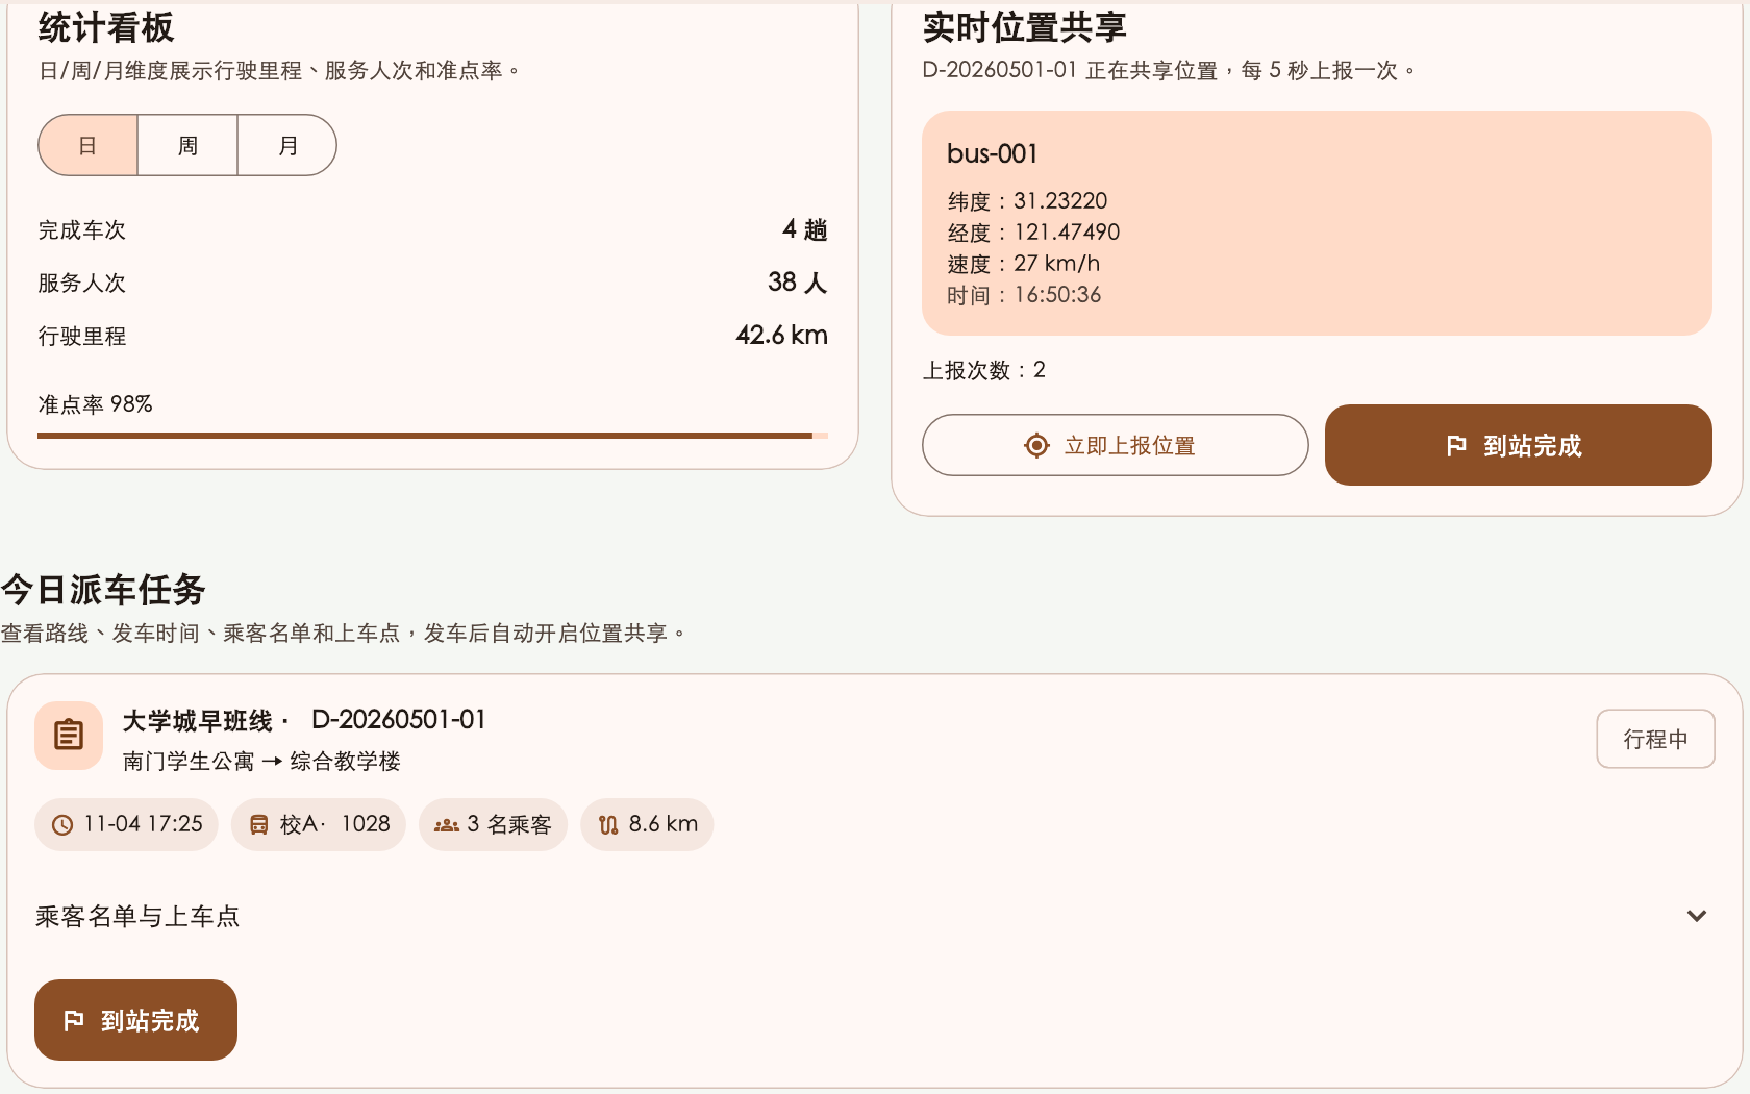
\includegraphics[width=\linewidth,height=0.64\textheight,keepaspectratio]{figures/driver.pdf}
\caption{司机任务行程中与模拟位置上报的运行界面}\label{fig:driver-screen}
\end{figure}

司机工作台将任务执行状态与位置共享状态放在同一页面。任务卡片提供路线、发车时间和乘客信息，司机开始任务后可看到当前车辆、坐标、速度和最近上报时间；到站完成后共享停止，任务状态相应改变。

本阶段已建立任务状态与模拟位置记录联动的基础，并完成日、周、月统计展示。后续将以共享服务端为连接点，统一后台确认方案与司机任务的数据来源，再逐步接入真实定位与通信；同时完善乘客预约、后台调度和司机执行之间的数据一致性验证。

\end{document}
